% ----------------------------------------------------------------- %
%             The Speech Signal Processing Toolkit (SPTK)           %
%             developed by SPTK Working Group                       %
%             http://sp-tk.sourceforge.net/                         %
% ----------------------------------------------------------------- %
%                                                                   %
%  Copyright (c) 1984-2007  Tokyo Institute of Technology           %
%                           Interdisciplinary Graduate School of    %
%                           Science and Engineering                 %
%                                                                   %
%                1996-2017  Nagoya Institute of Technology          %
%                           Department of Computer Science          %
%                                                                   %
% All rights reserved.                                              %
%                                                                   %
% Redistribution and use in source and binary forms, with or        %
% without modification, are permitted provided that the following   %
% conditions are met:                                               %
%                                                                   %
% - Redistributions of source code must retain the above copyright  %
%   notice, this list of conditions and the following disclaimer.   %
% - Redistributions in binary form must reproduce the above         %
%   copyright notice, this list of conditions and the following     %
%   disclaimer in the documentation and/or other materials provided %
%   with the distribution.                                          %
% - Neither the name of the SPTK working group nor the names of its %
%   contributors may be used to endorse or promote products derived %
%   from this software without specific prior written permission.   %
%                                                                   %
% THIS SOFTWARE IS PROVIDED BY THE COPYRIGHT HOLDERS AND            %
% CONTRIBUTORS "AS IS" AND ANY EXPRESS OR IMPLIED WARRANTIES,       %
% INCLUDING, BUT NOT LIMITED TO, THE IMPLIED WARRANTIES OF          %
% MERCHANTABILITY AND FITNESS FOR A PARTICULAR PURPOSE ARE          %
% DISCLAIMED. IN NO EVENT SHALL THE COPYRIGHT OWNER OR CONTRIBUTORS %
% BE LIABLE FOR ANY DIRECT, INDIRECT, INCIDENTAL, SPECIAL,          %
% EXEMPLARY, OR CONSEQUENTIAL DAMAGES (INCLUDING, BUT NOT LIMITED   %
% TO, PROCUREMENT OF SUBSTITUTE GOODS OR SERVICES; LOSS OF USE,     %
% DATA, OR PROFITS; OR BUSINESS INTERRUPTION) HOWEVER CAUSED AND ON %
% ANY THEORY OF LIABILITY, WHETHER IN CONTRACT, STRICT LIABILITY,   %
% OR TORT (INCLUDING NEGLIGENCE OR OTHERWISE) ARISING IN ANY WAY    %
% OUT OF THE USE OF THIS SOFTWARE, EVEN IF ADVISED OF THE           %
% POSSIBILITY OF SUCH DAMAGE.                                       %
% ----------------------------------------------------------------- %
\hypertarget{spec}{}
\name{spec}{transform real sequence to log spectrum}{signal processing}

\begin{synopsis}
 \item[spec]   [ --l $L$ ] [ --m $M$ ] [ --n $N$ ] [ --z {\em zfile} ]
               [ --p {\em pfile} ]
 \item[\ ~~~~] [ --e $e$ ] [ --E $E$ ] [ --o $O$ ] [ {\em infile} ]
\end{synopsis}

\begin{qsection}{DESCRIPTION}
{\em spec} computes the log spectrum magnitude of framed windowed input data 
from {\em infile} (or standard input), 
and sends the result to standard output.

Alternatively, given the poles (--p {\em pfile} option) 
and zeroes (--z {\em zfile} option) of a digital filter, 
{\em spec} computes the frequency response of that filter.

The output format is specified by the --y option.

If the input sequence is given by
\begin{displaymath}
  x(0), x(1), \dots, x(L-1)
\end{displaymath}
and the FFT algorithm is used to evaluate
\begin{align}
  X_k &= X(e^{j\omega}) \left|
	\begin{array}{c}
	\\
        \omega=\frac{2\pi k}{L}
	\end{array}
    \right. \notag \\
          &= \sum_{m=0}^{L-1}x(m)e^{-j\omega m} \left|
	\begin{array}{c}
	\\
        \omega=\frac{2\pi\, k}{L}
	\end{array}
    \right., \qquad k=0,1,\dots,L-1 \notag
\end{align}
then if the {\bf --y} option is applied, the output will be
\begin{displaymath}
  Y_k=20\,\log_{10}\,|X_k|,\qquad k=0,1,\dots,L/2
\end{displaymath}
The output data corresponds to angular frequencies varying from $0\sim \pi$.
Input and output data are in float format.
\par
If the {\bf --p} and {\bf --z} options are assigned
then the phase of the corresponding filter related to
the assigned coefficients is calculated
\footnote{
In this case the phase is not evaluated from the filter
impulse response, the phase is evaluated from
the difference between the numerator and denominator phases}.
\end{qsection}

\begin{options}
	\argm{l}{L}{FFT window length\\
                    $L$ must be power of 2}{256}
	\argm{m}{M}{order of MA part\\
			In the case where the number of input data
                        values is less then $M+1$, then $M$ is made
                        equal to the number of input data values $-1$.
                        You don't need to assign a value to $M$
                        in case there is no need to for the data to be analyzed
                        in blocks of size $M+1$.}{0}
	\argm{n}{N}{order of AR part\\
                        Similarly to the --m option,
			in the case where the number of input data
                        values is less then $N+1$, then $N$ is made
                        equal to the number of input data values $-1$.
                        You don't need to assign a value to $N$
                        in case there is no need to for the data to be analyzed
                        in blocks of size $N+1$.}{0}
	\argm{z}{zfile}{MA coefficients filename\\
			The {\em zfile} should contain the following structure in
                        float format:\\
			\hspace*{2ex}$b(0), b(1), \dots, b(N)$\\[-1ex]}{NULL}
	\argm{p}{pfile}{AR coefficients filename\\
			The {\em pfile} should contain the following structure in
                        float format:\\
			\hspace*{2ex}$K, a(1), \dots, a(M)$\\[-1ex]}{NULL}
	\argm{e}{e}{small value for calculating $\log()$}{0.0}
	\argm{E}{E}{floor in db calculated per frame}{N/A}
	\argm{o}{O}{output format\\
			\begin{tabular}{lll} \\[-1ex]
			$O=0$ & ~~~$20\times\log |X_k|$ & $k=0,1,\dots,L/2$\\
			$O=1$ & ~~~$\ln |X_k|$ & $k=0,1,\dots,L/2$\\
			$O=2$ & ~~~$|X_k|$ & $k=0,1,\dots,L/2$\\
			$O=3$ & ~~~$|X_k|^{2}$ & $k=0,1,\dots,L/2$\\             
			\end{tabular} \\\hspace*{\fill}}{0}
	\desc{The contents of {\em pfile} and {\em zfile}
                        should be in a similar form to that used in
                        the {\em dfs} command.
			When only the {\bf --p} option is assigned,
                        the denominator is set to 1.
                        When only the {\bf --z} option is assigned,
                        the numerator and the gain $K$ are set to 1.
                        If neither {\bf --p} nor {\bf --z} are
                        assigned, data is read from the standard input.}
\end{options}

\begin{qsection}{EXAMPLE}
In the example below, a pulse train excitation is passed
through digital filter and Blackman window.
The log spectrum magnitude is, thus, evaluated and plotted
on the screen:
\begin{quote}
  \verb!train -p 50 | dfs -a 1 0.9 | window | spec | fdrw | xgr !
\end{quote}
\begin{center}
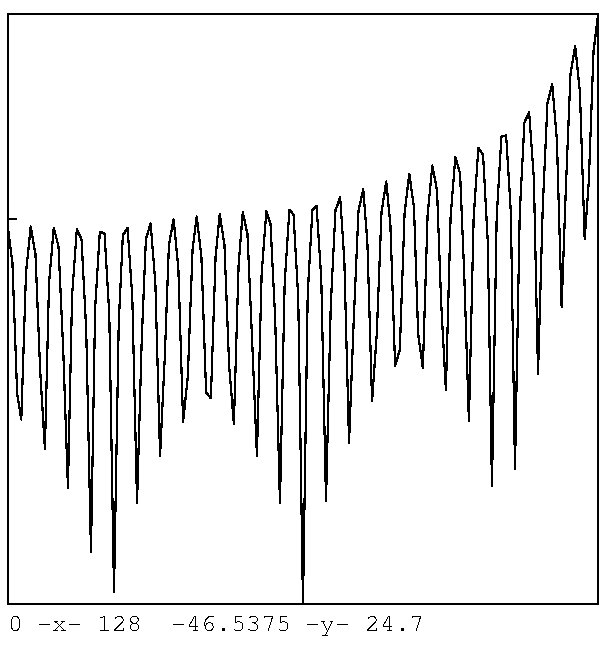
\includegraphics[width=4cm]{fig/spec_1.pdf}
\end{center}
\par
This example evaluates the frequency response of
a digital filter with coefficients specified in {\em data.p and data.z}
in float format:
\begin{quote}
  \verb!spec -p data.p -z data.z | fdrw | xgr !
\end{quote}
\begin{center}
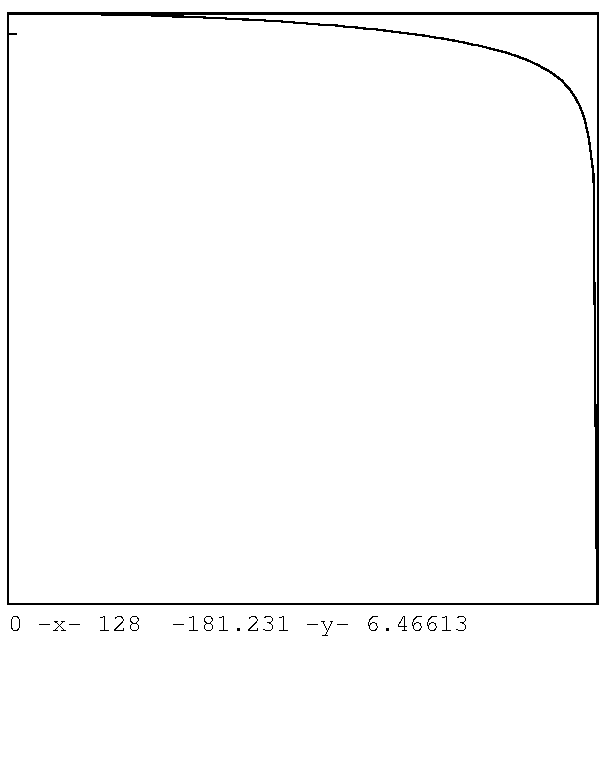
\includegraphics[width=4cm]{fig/spec_2.pdf}
\end{center}

A similar result can be obtained with the following command,
 for a stable filter:
\begin{quote}
  \verb!impulse | dfs -p data.p -z data.z | spec | fdrw | xgr !
\end{quote}
\begin{center}
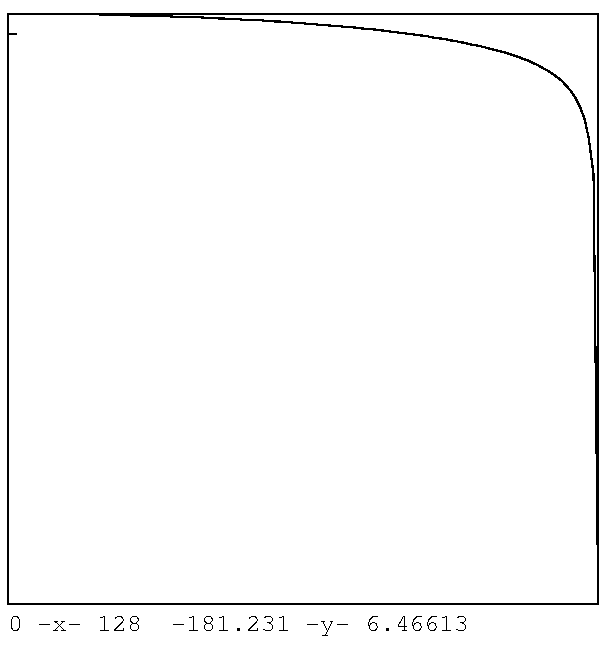
\includegraphics[width=4cm]{fig/spec_3.pdf}
\end{center}
Also, in the following example, the floor value is set as -30 dB per frame by using the -E option.
 \begin{quote}
 \verb! spec -E -30 data.f | fdrw | xgr !
 \end{quote}
\begin{center}
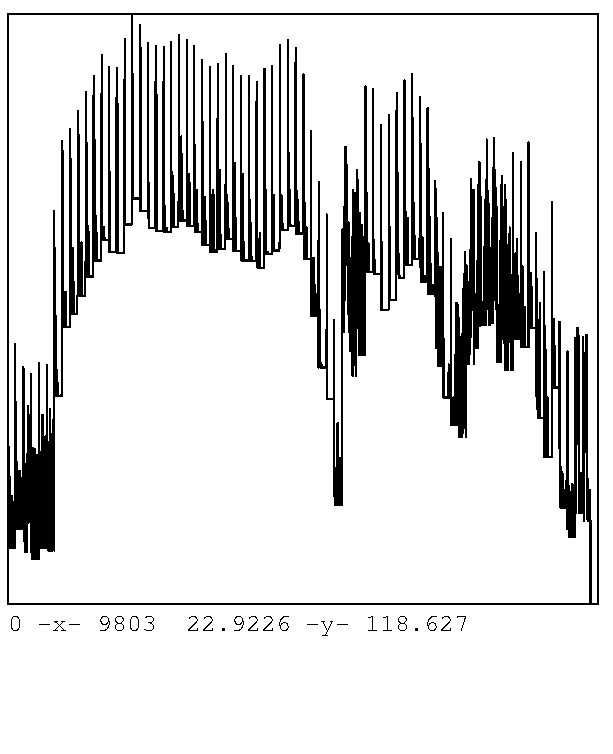
\includegraphics[width=4cm]{fig/spec_4.pdf}
\end{center}


\end{qsection}

\begin{qsection}{NOTICE}
\begin{itemize}
\item Value of $e$ must be $e \geq 0$.
\item Value of $E$ must be $E < 0$.
\end{itemize}
\end{qsection}

\begin{qsection}{SEE ALSO}
\hyperlink{phase}{phase},
\hyperlink{fft}{fft},
\hyperlink{fftr}{fftr},
\hyperlink{dfs}{dfs}
\end{qsection}
